% !TeX spellcheck = de_DE
\section{Strategien zur Datenmigration}
%TODO Tobias

Strategien zur Migration von Daten lassen sich in zwei Dimensionen unterteilen. Eine Dimension dieser Strategien bezieht sich auf die Datenhaltung selbst. Die zweite Dimension befasst sich mit der Nutzung dieser Daten auf Anwendungsebene \citep{henrard-2002}. Eine Unterscheidung erfolgt dabei jeweils anhand von Unterkategorien.
\lb
Die Dimension der Datenhaltung befasst sich mit Strategien zur Transformation und Migration von Daten auf Ebene von Datenstrukturen. Unterschieden werden kann dabei auf physischer und konzeptueller Ebene.
\lb
Eine physische Migration von Daten schlie"st einen Wechsel des Medium ein. Daten werden dabei von einem physischen Speicher auf einen weiteren "ubertragen. Dies schlie"st auch eine grunds"atzliche "Ubersetzung von Daten aus einer Technologie auf eine andere ein. Die Logik der Daten wird dabei nicht hinterfragt \citep{henrard-2002}. 
\lb
Die konzeptuelle Migration beinhaltet Ver"anderungen im Bezug auf Datenbank-Schemata oder Dateiformate. Vorhandene Daten m"ussen konzeptuell neu gegliedert werden. Dies ist etwa notwendig, wenn Gesch"aftsprozesse und zugrundeliegende Daten ver"andert werden oder die Technologie zur Datensicherung ausgetauscht wird. Der Wechsel von einem relationalen auf ein objektorientiertes Datenbank-Schema ist ein Beispiel dieser Kategorie.
\lb
%TODO Diese Auflistung weiter oben, ist wichtig
Die Grundlegenden Bestandteile der Datenmigration gliedern sich in drei elementare T"atigkeiten \citep{henrard-2002}.

\begin{itemize}
	\item \textbf{Konvertierung des Datenhaltungs-Schemata} \\
	Erkennen und Analysieren von vorhandenen Schemata und Datenformaten. Auf Basis der existierenden Datenformate wird unter Umst"anden eine Neukonzeptionierung der Formate vorgenommen. Anpassungen m"ussen die Erhaltung der bereits vorhandenen Datenber"ucksichtigen und neue Schemata auf Basis der Ziel-Technologie etablieren.
	\item \textbf{Konvertierung der Daten} \\
	Ist die Konvertierung der Schemata erfolgt, m"ussen die Daten selbst in das neue Format gebracht werden. Eine Automatisierung durch Umkopieren der Daten vom alten in das neu Format verk"orpert die Konvertierung.
	\item \textbf{Anpassung der Anwendung} \\
	Sind Daten und Schemata konvertiert, m"ussen angrenzende Softwaresystem angepasst werden. Anwendungen, welche alte Datenformate und -technologien nutzen, m"ussen auf die Nutzung der neuen Formate hin angepasst werden.
\end{itemize}

\begin{figure}[h!]
	\centering
	\caption{Kategorisierung Strategien der Datenmigration}
	\label{pic:strategien}
	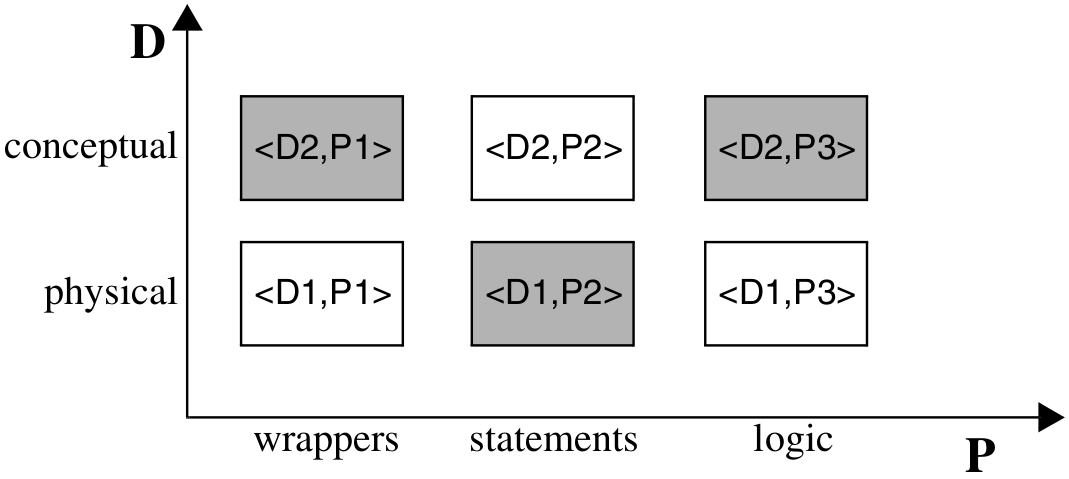
\includegraphics[width=0.9\textwidth]{../images/strategies_fig_01.png} \\
	\tiny Quelle: \citep{henrard-2002}, Abbildung 1
\end{figure}

Aus der gegebenen Kategorisierung von Migrationsstrategien leiten sich somit sechs unterschiedliche Strategien (Siehe Abbildung \ref{pic:strategien}) ab.

\subsection{Physische Konvertierung}

\begin{figure}[h!]
	\centering
	\caption{Physische Konvertierung}
	\label{pic:conversion_physical}
	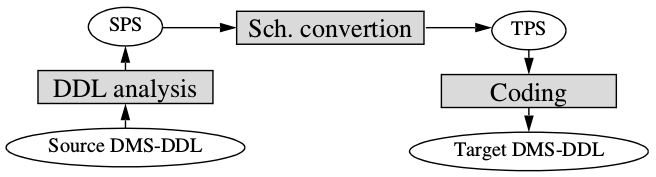
\includegraphics[width=0.9\textwidth]{../images/strategies_fig_02a.png} \\
	\tiny Quelle: \citep{henrard-2002}, Abbildung 2
\end{figure}

\subsection{Konzeptuelle Konvertierung}

\begin{figure}[h!]
	\centering
	\caption{Konzeptuelle Konvertierung}
	\label{pic:conversion_conceptual}
	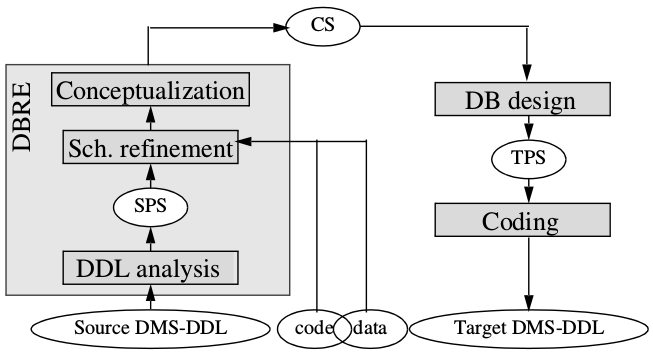
\includegraphics[width=0.9\textwidth]{../images/strategies_fig_02b.png} \\
	\tiny Quelle: \citep{henrard-2002}, Abbildung 2
\end{figure}


%Jeweils:
%\begin{itemize}
%	\item Wessen Aufgabe ist die Migration?
%	\item Auswirkung auf umliegende Systeme (Folgen)?
%	\item Vorteile?
%	\item Nachteile?
%\end{itemize}
%
%\subsection{Storage Migration}
%
%\begin{itemize}
%	\item Neue physische Hardware
%	\item Jemand kauft einen neuen Server -> unter Umst"anden neues Schreiben der Daten auf physischen Datentr"ager
%\end{itemize}
%
%\subsection{Database Migration}
%
%\begin{itemize}
%	\item Neue Version von DBMS etc.
%	\item Etwa Upgrade Oracle 7.0 -> 11.0: Unterschiedliche Verwaltung von Speicher und Administration
%\end{itemize}
%
%\subsection{Application Migration}
%
%\begin{itemize}
%	\item Neues DB-System etc. (Etwa Oracle -> MSSql)
%	\item Andere Formate, Statements, Zugriffe etc.
%\end{itemize}
%
%\subsection{Business Process Migration}
%
%\begin{itemize}
%	\item Anpassung von Daten an Business-Prozesse
%	\item Etwa Spaltung eines Unternehmens: Vorher alle Daten in einer DB, nach Spaltung geh"oren die Daten rechtlich entweder dem einen oder anderen Unternehmen und m"ussen entsprechend getrennt werden.
%	\item Datenhaltung bildet von Business-Prozesse ab und muss entsprechend migriert werden
%\end{itemize}